\documentclass[11pt,a4paper]{article}

\usepackage[top=20mm,bottom=26mm,left=20mm,right=20mm,headheight=15pt,footskip=12mm]{geometry}

\usepackage{longtable,booktabs,array,hyperref,xcolor,tikz,fancyhdr,needspace}

\usepackage{fontspec,xeCJK}

\setmainfont[Ligatures=TeXOff]{Times New Roman}

\setsansfont[Ligatures=TeXOff]{Times New Roman}

\setmonofont[Ligatures=TeXOff,WordSpace={1,1,1}]{Times New Roman}

\setCJKmainfont{Noto Serif CJK SC}

\setCJKsansfont{Noto Serif CJK SC}

\setCJKmonofont{Noto Serif CJK SC}

\newfontfamily\vulcanmathsymbols{Noto Serif CJK SC}

\XeTeXgenerateactualtext=1

\definecolor{vulcan}{HTML}{BB3E23}

\definecolor{vulcanblue}{HTML}{1B4F72}

\renewcommand{\thesection}{\Roman{section}}

\renewcommand{\thesubsection}{\Alph{subsection}}

\pgfdeclarelayer{connections}\pgfdeclarelayer{edge labels}\pgfsetlayers{connections,main,edge labels}

\hypersetup{hidelinks}

\newcolumntype{L}[1]{>{\raggedright\arraybackslash\hspace{0pt}}p{#1}}

\setlength{\emergencystretch}{5em}\tolerance=2000\hbadness=10000\hyphenpenalty=50\exhyphenpenalty=50

\setlength{\parindent}{0pt}\setlength{\parskip}{5pt}

\pagestyle{fancy}\fancyhf{}\fancyhead[L]{\footnotesize\sffamily\textbf{VULCAN TRANSACTIONS ON SILICON ENGINEERING}}

\fancyhead[R]{\footnotesize\sffamily RTL Microarchitecture \& Silicon Signoff}\fancyfoot[C]{\footnotesize\sffamily Page \thepage}

\begin{document}

{\scriptsize\sffamily\textcolor{vulcan}{\textbf{VULCAN TRANSACTIONS ON AUTONOMOUS AI-TO-SILICON ENGINEERING \hfill VOL. 2026 \textperiodcentered{} ARCHITECTURAL SIGNOFF PAPER}}\par}

\vspace{1pt}\textcolor{vulcan}{\rule{\textwidth}{1.2pt}}\vspace{4pt}

\begin{center}

{\sffamily\LARGE\bfseries BELLOWS-L2: Hardware LZ4 Compression and Decompression\par}\vspace{3pt}

{\small\sffamily\textbf{Sufeng Guo (\allowbreak{}sufeng\_\allowbreak{}guo@smail.nju.edu.cn)\allowbreak{}} \textperiodcentered{} Microsoft Research Asia \textperiodcentered{} Technical Design and Verification Report\par}\vspace{1pt}

{\scriptsize\sffamily\textcolor{black!75}{Silicon Platform: Intel Arria 10 GX (\texttt{10AX115N3F40E2SG}) PCIe Gen3x8 \textperiodcentered{} Toolchain: Icarus Verilog 12.0 / Yosys 0.33 / Quartus Prime 17.1 STA \textperiodcentered{} 29 October 2026 (\allowbreak{}2026-10-29 21:29 UTC+\allowbreak{}8 Beijing Time)\allowbreak{}}\par}

\end{center}\vspace{2pt}

\renewcommand{\abstractname}{\textcolor{vulcanblue}{Abstract}}\begin{abstract}\noindent BELLOWS-L2 combines a block-buffered hardware LZ4 compressor with the preserved BELLOWS-L1 streaming decoder. Byte-wide interfaces support independent simultaneous compression and decompression or selectable internal compress-then-decompress operation. Registered four-byte hash lookup,\allowbreak{} literal-anchor buffering and a token emitter implement actual match compression. Software-vs-Hardware numerical comparison passed all 18 capacity/\allowbreak{}seed configurations with byte-exact recovery. Each of six required repetitive fixtures achieved compression ratio below 1.0: 4096-byte inputs produced 26–282 encoded bytes,\allowbreak{} and 65536-byte inputs produced 267–523 encoded bytes. These results establish agreement for executed cases,\allowbreak{} not exhaustive mathematical proof. [\allowbreak{}E1187,\allowbreak{} E1641]\allowbreak{} Native L1 RTL timing lint,\allowbreak{} designated L1.5 in the work order,\allowbreak{} passed. L2 Intel Quartus Prime 17.1 TimeQuest post-fit STA reported WNS\_\allowbreak{}setup =\allowbreak{} +\allowbreak{}3.405 ns at a 10.0 ns clock period on Arria 10 GX 10AX115N2F45E1SG. This standalone-IP configuration uses virtual pins except for clk and only a clock constraint,\allowbreak{} establishing internal timing closure rather than board-level interface timing. L3 recorded three consecutive deterministic physical FPGA HIL passes; retained HIL output documents register diagnostics,\allowbreak{} while portable simulations support the payload-level numerical comparisons. [\allowbreak{}E1642,\allowbreak{} E1643,\allowbreak{} E1644]\allowbreak{}\par\vspace{2pt}{\scriptsize\textbf{\textcolor{vulcanblue}{Index Terms---}}Autonomous RTL Generation, SystemVerilog, Intel Arria 10 GX FPGA, TimeQuest 100~MHz+ Timing Closure, PCIe Gen3x8 Hardware-in-the-Loop (HIL), Bit-Exact Fixed-Point Verification.}\end{abstract}\vspace{2pt}

\needspace{5\baselineskip}\section{Architecture and design rationale}

The single-clock design retains the three parent decoder modules byte-for-byte and adds a separate compressor hierarchy. Compression collects a complete bounded block before searching and encoding. Buffering permits overlap-safe comparison against original bytes and exact literal-only fallback before encoded output becomes externally visible. Synchronous memories and serial comparison trade throughput and latency for bounded combinational depth. Blocks below are arranged row-major in three columns. [\allowbreak{}E001–E010]\allowbreak{}

\begin{center}\begin{minipage}{\textwidth}\centering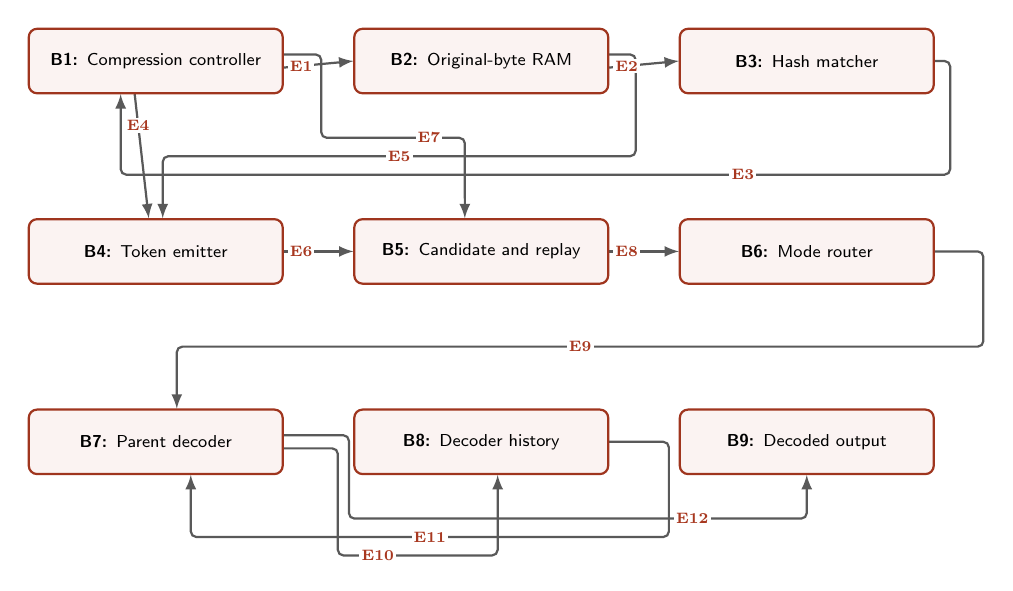
\begin{tikzpicture}[scale=0.78,transform shape,every node/.style={font=\footnotesize\sffamily},>=latex]

\node[draw=vulcan!85!black,thick,rounded corners=3pt,fill=vulcan!6,text width=3.9cm,minimum height=1.05cm,align=center] (b0) at (0.0,0.0) {\textbf{B1:} Compression controller};

\node[draw=vulcan!85!black,thick,rounded corners=3pt,fill=vulcan!6,text width=3.9cm,minimum height=1.05cm,align=center] (b1) at (5.3,0.0) {\textbf{B2:} Original-byte RAM};

\node[draw=vulcan!85!black,thick,rounded corners=3pt,fill=vulcan!6,text width=3.9cm,minimum height=1.05cm,align=center] (b2) at (10.6,0.0) {\textbf{B3:} Hash matcher};

\node[draw=vulcan!85!black,thick,rounded corners=3pt,fill=vulcan!6,text width=3.9cm,minimum height=1.05cm,align=center] (b3) at (0.0,-3.1) {\textbf{B4:} Token emitter};

\node[draw=vulcan!85!black,thick,rounded corners=3pt,fill=vulcan!6,text width=3.9cm,minimum height=1.05cm,align=center] (b4) at (5.3,-3.1) {\textbf{B5:} Candidate and replay};

\node[draw=vulcan!85!black,thick,rounded corners=3pt,fill=vulcan!6,text width=3.9cm,minimum height=1.05cm,align=center] (b5) at (10.6,-3.1) {\textbf{B6:} Mode router};

\node[draw=vulcan!85!black,thick,rounded corners=3pt,fill=vulcan!6,text width=3.9cm,minimum height=1.05cm,align=center] (b6) at (0.0,-6.2) {\textbf{B7:} Parent decoder};

\node[draw=vulcan!85!black,thick,rounded corners=3pt,fill=vulcan!6,text width=3.9cm,minimum height=1.05cm,align=center] (b7) at (5.3,-6.2) {\textbf{B8:} Decoder history};

\node[draw=vulcan!85!black,thick,rounded corners=3pt,fill=vulcan!6,text width=3.9cm,minimum height=1.05cm,align=center] (b8) at (10.6,-6.2) {\textbf{B9:} Decoded output};

\begin{pgfonlayer}{connections}

\draw[->,thick,black!65] ([yshift=-0.107cm]b0.east) -- coordinate[pos=0.25] (e0) ([yshift=0.000cm]b1.west);

\draw[->,thick,black!65] ([yshift=-0.107cm]b1.east) -- coordinate[pos=0.25] (e1) ([yshift=0.000cm]b2.west);

\draw[->,thick,black!65,rounded corners=2pt] ([yshift=0.000cm]b2.east) -- (12.935,0.000) -- (12.935,-1.850) -- coordinate[pos=0.25] (e2) (-0.571,-1.850) -- ([xshift=-0.571cm]b0.south);

\draw[->,thick,black!65] ([xshift=-0.343cm]b0.south) -- coordinate[pos=0.25] (e3) ([xshift=-0.114cm]b3.north);

\draw[->,thick,black!65,rounded corners=2pt] ([yshift=0.107cm]b1.east) -- (7.815,0.107) -- (7.815,-1.550) -- coordinate[pos=0.50] (e4) (0.114,-1.550) -- ([xshift=0.114cm]b3.north);

\draw[->,thick,black!65] ([yshift=0.000cm]b3.east) -- coordinate[pos=0.25] (e5) ([yshift=0.000cm]b4.west);

\draw[->,thick,black!65,rounded corners=2pt] ([yshift=0.107cm]b0.east) -- (2.695,0.107) -- (2.695,-1.250) -- coordinate[pos=0.75] (e6) (5.033,-1.250) -- ([xshift=-0.267cm]b4.north);

\draw[->,thick,black!65] ([yshift=0.000cm]b4.east) -- coordinate[pos=0.25] (e7) ([yshift=0.000cm]b5.west);

\draw[->,thick,black!65,rounded corners=2pt] ([yshift=0.000cm]b5.east) -- (13.475,-3.100) -- (13.475,-4.650) -- coordinate[pos=0.50] (e8) (0.343,-4.650) -- ([xshift=0.343cm]b6.north);

\draw[->,thick,black!65,rounded corners=2pt] ([yshift=-0.107cm]b6.east) -- (2.965,-6.307) -- (2.965,-8.050) -- coordinate[pos=0.25] (e9) (5.567,-8.050) -- ([xshift=0.267cm]b7.south);

\draw[->,thick,black!65,rounded corners=2pt] ([yshift=0.000cm]b7.east) -- (8.355,-6.200) -- (8.355,-7.750) -- coordinate[pos=0.50] (e10) (0.571,-7.750) -- ([xshift=0.571cm]b6.south);

\draw[->,thick,black!65,rounded corners=2pt] ([yshift=0.107cm]b6.east) -- (3.145,-6.093) -- (3.145,-7.450) -- coordinate[pos=0.75] (e11) (10.600,-7.450) -- ([xshift=0.000cm]b8.south);

\end{pgfonlayer}

\begin{pgfonlayer}{edge labels}

\node[fill=white,inner sep=1pt,font=\scriptsize\bfseries,text=vulcan!90!black] at (e0) {E1};

\node[fill=white,inner sep=1pt,font=\scriptsize\bfseries,text=vulcan!90!black] at (e1) {E2};

\node[fill=white,inner sep=1pt,font=\scriptsize\bfseries,text=vulcan!90!black] at (e2) {E3};

\node[fill=white,inner sep=1pt,font=\scriptsize\bfseries,text=vulcan!90!black] at (e3) {E4};

\node[fill=white,inner sep=1pt,font=\scriptsize\bfseries,text=vulcan!90!black] at (e4) {E5};

\node[fill=white,inner sep=1pt,font=\scriptsize\bfseries,text=vulcan!90!black] at (e5) {E6};

\node[fill=white,inner sep=1pt,font=\scriptsize\bfseries,text=vulcan!90!black] at (e6) {E7};

\node[fill=white,inner sep=1pt,font=\scriptsize\bfseries,text=vulcan!90!black] at (e7) {E8};

\node[fill=white,inner sep=1pt,font=\scriptsize\bfseries,text=vulcan!90!black] at (e8) {E9};

\node[fill=white,inner sep=1pt,font=\scriptsize\bfseries,text=vulcan!90!black] at (e9) {E10};

\node[fill=white,inner sep=1pt,font=\scriptsize\bfseries,text=vulcan!90!black] at (e10) {E11};

\node[fill=white,inner sep=1pt,font=\scriptsize\bfseries,text=vulcan!90!black] at (e11) {E12};

\end{pgfonlayer}

\end{tikzpicture}\par\vspace{3pt}

{\small\textbf{Figure 1:} Top-level microarchitectural functional block map and directed inter-module bus topology.}\end{minipage}\end{center}

{\small\renewcommand{\arraystretch}{1.18}\begin{longtable}{@{}L{0.24\textwidth}|L{0.7\textwidth}@{}}\toprule

\textbf{Block} & \textbf{Responsibility}\\\midrule\endhead

B1: Compression controller & bellows\_\allowbreak{}l2\_\allowbreak{}compressor owns collection,\allowbreak{} framing errors,\allowbreak{} discard,\allowbreak{} block length,\allowbreak{} literal anchor,\allowbreak{} memory-port arbitration and completion status.\\[2pt]\hline

B2: Original-byte RAM & bellows\_\allowbreak{}l2\_\allowbreak{}literal\_\allowbreak{}buffer stores MAX\_\allowbreak{}BLOCK\_\allowbreak{}BYTES bytes with synchronous reads: 65536 x 8 logical bits at default capacity.\\[2pt]\hline

B3: Hash matcher & bellows\_\allowbreak{}l2\_\allowbreak{}hash\_\allowbreak{}match acquires four-byte keys,\allowbreak{} registers hash lookup,\allowbreak{} validates candidates and extends matches serially. Storage includes 256 positions of 16 bits and 256 validity bits.\\[2pt]\hline

B4: Token emitter & bellows\_\allowbreak{}l2\_\allowbreak{}emitter accepts sequence descriptors and registers tokens,\allowbreak{} extensions,\allowbreak{} literals and little-endian offsets.\\[2pt]\hline

B5: Candidate and replay & Controller-owned synchronous RAM stores 2*\allowbreak{}MAX\_\allowbreak{}BLOCK\_\allowbreak{}BYTES+\allowbreak{}16 encoded bytes,\allowbreak{} or 131088 bytes by default. Completed-size comparison selects candidate replay or literal-only regeneration.\\[2pt]\hline

B6: Mode router & bellows\_\allowbreak{}l2\_\allowbreak{}top directs compressed data externally or into the decoder. Independent mode permits both lanes to operate concurrently.\\[2pt]\hline

B7: Parent decoder & Unmodified bellows\_\allowbreak{}l1\_\allowbreak{}top parses raw LZ4 and reconstructs bytes while retaining parent framing,\allowbreak{} error and status behavior.\\[2pt]\hline

B8: Decoder history & Unmodified bellows\_\allowbreak{}l1\_\allowbreak{}history supplies synchronous 65536-byte rolling storage. History ownership is invalidated between blocks.\\[2pt]\hline

B9: Decoded output & Unmodified bellows\_\allowbreak{}l1\_\allowbreak{}output stages pending and presented bytes,\allowbreak{} identifies the final byte and preserves held output under backpressure.\\[2pt]\hline

\bottomrule\end{longtable}}

{\small\renewcommand{\arraystretch}{1.18}\begin{longtable}{@{}L{0.24\textwidth}|L{0.7\textwidth}@{}}\toprule

\textbf{Directed relationship} & \textbf{Meaning}\\\midrule\endhead

E1: B1 to B2 & Accepted raw-byte writes\\[2pt]\hline

E2: B2 to B3 & Registered search bytes\\[2pt]\hline

E3: B3 to B1 & Match descriptors and done\\[2pt]\hline

E4: B1 to B4 & Literal-span and match descriptors\\[2pt]\hline

E5: B2 to B4 & Registered literal bytes\\[2pt]\hline

E6: B4 to B5 & Encoded sequence bytes\\[2pt]\hline

E7: B1 to B5 & Size selection and replay control\\[2pt]\hline

E8: B5 to B6 & Compressed ready/\allowbreak{}valid stream\\[2pt]\hline

E9: B6 to B7 & Selected external or internal stream\\[2pt]\hline

E10: B7 to B8 & History writes and read requests\\[2pt]\hline

E11: B8 to B7 & Registered history response\\[2pt]\hline

E12: B7 to B9 & Decoded candidates and finish\\[2pt]\hline

\bottomrule\end{longtable}}

\needspace{9\baselineskip}\section{Interfaces and configuration}

{\small\renewcommand{\arraystretch}{1.18}\begin{longtable}{@{}L{0.21\textwidth}|L{0.12\textwidth}|L{0.12\textwidth}|L{0.45\textwidth}@{}}\toprule

\textbf{Signal /\allowbreak{} group} & \textbf{Direction} & \textbf{Width} & \textbf{Contract}\\\midrule\endhead

clk; rst\_\allowbreak{}n; roundtrip\_\allowbreak{}enable & Input & 1 bit each & Rising-edge clock,\allowbreak{} asynchronous active-low reset and route selection. Change mode only during reset or when both lanes have no active block,\allowbreak{} output or outstanding status.\\[2pt]\hline

c\_\allowbreak{}s\_\allowbreak{}data; c\_\allowbreak{}s\_\allowbreak{}keep; c\_\allowbreak{}s\_\allowbreak{}valid; c\_\allowbreak{}s\_\allowbreak{}last; c\_\allowbreak{}s\_\allowbreak{}ready & Inputs: data,\allowbreak{} keep,\allowbreak{} valid,\allowbreak{} last; output: ready & Data 8 bits; others 1 bit & Raw compressor ingress. Normal bytes require keep=\allowbreak{}1. A sole keep=\allowbreak{}0,\allowbreak{}last=\allowbreak{}1 beat represents an empty block,\allowbreak{} with ignored data.\\[2pt]\hline

c\_\allowbreak{}m\_\allowbreak{}data; c\_\allowbreak{}m\_\allowbreak{}valid; c\_\allowbreak{}m\_\allowbreak{}last; c\_\allowbreak{}m\_\allowbreak{}ready & Outputs: data,\allowbreak{} valid,\allowbreak{} last; input: ready & Data 8 bits; others 1 bit & Raw-LZ4 compressed output. In internal round-trip mode all three outputs are zero and c\_\allowbreak{}m\_\allowbreak{}ready is ignored.\\[2pt]\hline

c\_\allowbreak{}status\_\allowbreak{}valid; c\_\allowbreak{}status\_\allowbreak{}error; c\_\allowbreak{}status\_\allowbreak{}ready & Outputs: valid,\allowbreak{} error; input: ready & Error 3 bits; others 1 bit & Held compressor completion. Status follows final output retirement or completed error discard; acknowledgement permits the next raw block.\\[2pt]\hline

d\_\allowbreak{}s\_\allowbreak{}data; d\_\allowbreak{}s\_\allowbreak{}valid; d\_\allowbreak{}s\_\allowbreak{}last; d\_\allowbreak{}s\_\allowbreak{}ready & Inputs: data,\allowbreak{} valid,\allowbreak{} last; output: ready & Data 8 bits; others 1 bit & External raw-LZ4 decoder ingress,\allowbreak{} without a keep signal. d\_\allowbreak{}s\_\allowbreak{}ready is zero during internal round-trip operation.\\[2pt]\hline

d\_\allowbreak{}m\_\allowbreak{}data; d\_\allowbreak{}m\_\allowbreak{}valid; d\_\allowbreak{}m\_\allowbreak{}last; d\_\allowbreak{}m\_\allowbreak{}ready & Outputs: data,\allowbreak{} valid,\allowbreak{} last; input: ready & Data 8 bits; others 1 bit & Recovered byte stream. Empty decoded blocks produce no output beat.\\[2pt]\hline

d\_\allowbreak{}status\_\allowbreak{}valid; d\_\allowbreak{}status\_\allowbreak{}error; d\_\allowbreak{}status\_\allowbreak{}ready & Outputs: valid,\allowbreak{} error; input: ready & Error 3 bits; others 1 bit & Preserved decoder completion channel. Both status channels remain independently observable and handshaken in either mode.\\[2pt]\hline

\bottomrule\end{longtable}}

{\small\renewcommand{\arraystretch}{1.18}\begin{longtable}{@{}L{0.22\textwidth}|L{0.21\textwidth}|L{0.49\textwidth}@{}}\toprule

\textbf{Parameter} & \textbf{Default} & \textbf{Meaning /\allowbreak{} supported values}\\\midrule\endhead

MAX\_\allowbreak{}BLOCK\_\allowbreak{}BYTES & 65536 & Integer capacity from 1 through 65536 inclusive,\allowbreak{} interpreted as an unsigned datapath limit. Values 0 and 65537 receive explicit fatal diagnostics before transactions. Capacities 1,\allowbreak{} 5,\allowbreak{} 13,\allowbreak{} 257,\allowbreak{} 4096 and 65536 were exercised. This parameter does not limit decoder output length. bellows\_\allowbreak{}l2\_\allowbreak{}compressor exposes the same parameter and compressor interfaces without their c\_\allowbreak{} prefix.\\[2pt]\hline

\bottomrule\end{longtable}}

\needspace{16\baselineskip}\section{Behavior and corner cases}

\subsection{Transfers,\allowbreak{} reset and completion}

Only pre-edge valid\&\&ready transfers a beat. Stalled senders hold valid and associated data,\allowbreak{} last and keep stable. All public outputs,\allowbreak{} including ready,\allowbreak{} are zero during reset. Reset abandons transactions and invalidates ownership without clearing large data arrays. Processing begins after collection closes in registered state,\allowbreak{} never through combinational input forwarding. No next compressor block is accepted until its status is acknowledged.

\needspace{10\baselineskip}\subsection{Frozen match search}

At ascending visited position p,\allowbreak{} compute h=\allowbreak{}b0 XOR rol8(\allowbreak{}b1,\allowbreak{}1)\allowbreak{} XOR rol8(\allowbreak{}b2,\allowbreak{}2)\allowbreak{} XOR rol8(\allowbreak{}b3,\allowbreak{}3)\allowbreak{},\allowbreak{} with eight-bit rotation. Each of 256 direct-mapped entries retains the latest inserted absolute position. Lookup reads the old entry before replacing it with p. Candidate q requires validity,\allowbreak{} q<p,\allowbreak{} offset 1..65535 and four equal bytes. Greedy extension permits overlap. Misses advance one byte; matches resume at their end without inserting skipped starts. Hash validity clears for every block.

\needspace{10\baselineskip}\subsection{End restrictions and encoding}

Blocks shorter than 13 bytes are literal-only. Otherwise match starts satisfy p<=\allowbreak{}N-12 and extensions end at or before N-5. Minimum match length is four,\allowbreak{} and every block ends with a literal-only sequence. Token nibbles encode min(\allowbreak{}literal\_\allowbreak{}length,\allowbreak{}15)\allowbreak{} and min(\allowbreak{}match\_\allowbreak{}length-4,\allowbreak{}15)\allowbreak{}; the final sequence has low nibble zero. Saturation requires repeated 255 extension bytes followed by a remainder 0..254,\allowbreak{} including a terminating zero when required. Emit literals before the nonzero offset,\allowbreak{} serialized low byte first,\allowbreak{} and then any match extension. Empty input encodes as 0x00.

\needspace{10\baselineskip}\subsection{Literal fallback}

Literal-only size is N+\allowbreak{}1,\allowbreak{} plus floor(\allowbreak{}(\allowbreak{}N-15)\allowbreak{}/\allowbreak{}255)\allowbreak{}+\allowbreak{}1 for N>=\allowbreak{}15. Retain the completed candidate only when strictly smaller; ties and larger candidates regenerate the exact literal-only encoding. Hardware computes extensions through registered subtraction rather than division. Verification checks the conservative candidate-storage bound.

\needspace{10\baselineskip}\subsection{Registered stages}

Four request/\allowbreak{}capture pairs acquire a key; separate stages register the hash,\allowbreak{} synchronous table response and candidate validation. Four further request/\allowbreak{}capture comparisons establish the minimum match. Extension uses check/\allowbreak{}request/\allowbreak{}capture stages. The emitter latches descriptors and registers bytes. Public replay uses request/\allowbreak{}load/\allowbreak{}hold states,\allowbreak{} inserting bubbles even with continuously ready output. Parent literals pass through commit staging; match bytes use synchronous history-read and commit states. Consumer stalls and variable search work prevent a fixed end-to-end cycle count.

\needspace{10\baselineskip}\subsection{Errors and recovery}

Compressor codes are 0 success,\allowbreak{} 5 capacity overflow and 6 malformed keep; other codes are reserved. First detected error wins,\allowbreak{} with malformed keep taking precedence when both arise on one beat. Error blocks emit no compressed output and drain through accepted last before status. Decoder codes remain 0 success,\allowbreak{} 1 truncation,\allowbreak{} 2 zero offset,\allowbreak{} 3 unavailable history and 4 length overflow,\allowbreak{} preserving valid-prefix output and subsequent recovery.

\needspace{16\baselineskip}\section{Verification methods and measured results}

\subsection{Software-vs-Hardware numerical comparison and lossless recovery}

\textbf{Method.} Independent Python raw-LZ4 parser and direct-sequence generator; actual Icarus and Verilator behavior checks. Six capacities crossed with seeds 1,\allowbreak{}17,\allowbreak{}89.

\textbf{Result.} 18/\allowbreak{}18 matrix cells passed. The ledger records 508 independently parsed compressed blocks,\allowbreak{} 504 hardware-compress/\allowbreak{}hardware-decompress cases and 80 internal-round-trip blocks. Complete-byte comparisons reported zero mismatches. Coverage counters include 1275086 compressor-reference bytes and 1770235 decoder-reference bytes,\allowbreak{} including repeated test traffic.

{\small Evidence: E011,\allowbreak{} E012,\allowbreak{} E1187,\allowbreak{} E1641}

\needspace{12\baselineskip}\subsection{Each structured fixture has ratio below 1.0 and real matches}

\textbf{Method.} Measure actual RTL encoded lengths and independently parse matches; run each fixture under all three seeds. Ratio is encoded/\allowbreak{}input bytes,\allowbreak{} excluding status.

\textbf{Result.} At N=\allowbreak{}4096: repeated A 26/\allowbreak{}4096=\allowbreak{}0.00634765625; ABCD 29/\allowbreak{}4096=\allowbreak{}0.007080078125; byte ramp 282/\allowbreak{}4096=\allowbreak{}0.06884765625. At N=\allowbreak{}65536: A 267/\allowbreak{}65536; ABCD 270/\allowbreak{}65536; byte ramp 523/\allowbreak{}65536. All six pass separately,\allowbreak{} contain matches and retain five final literals.

{\small Evidence: E1187,\allowbreak{} E1641}

\needspace{12\baselineskip}\subsection{Backpressure,\allowbreak{} boundaries and recovery}

\textbf{Method.} Public-pin assertions,\allowbreak{} independent ingress/\allowbreak{}egress/\allowbreak{}status stalls,\allowbreak{} simultaneous duplex traffic,\allowbreak{} resets and directed format/\allowbreak{}history cases.

\textbf{Result.} Passed held-final and held-status checks on applicable channels,\allowbreak{} 377 exact fallback comparisons,\allowbreak{} 152 malformed/\allowbreak{}post-error-recovery cases,\allowbreak{} offset-65535 and history-wrap cases,\allowbreak{} output beyond 65536 bytes,\allowbreak{} extension boundaries and reset coverage. Illegal capacity endpoints were explicitly rejected.

{\small Evidence: E011,\allowbreak{} E015,\allowbreak{} E1187,\allowbreak{} E1641}

\needspace{12\baselineskip}\subsection{Defect sensitivity}

\textbf{Method.} Compile and execute three disposable synthesizable RTL mutants without changing expected results.

\textbf{Result.} Offset corruption reached ZERO\_\allowbreak{}OFFSET rejection; trailing-limit violation reached TRAILING\_\allowbreak{}FIVE\_\allowbreak{}LITERALS rejection; stalled-output corruption reached HELD\_\allowbreak{}C\_\allowbreak{}OUTPUT rejection. Compilation failure or timeout was not counted as detection.

{\small Evidence: E1187,\allowbreak{} E1641}

\needspace{12\baselineskip}\subsection{Synthesizable hierarchy and bounded reproduction}

\textbf{Method.} Real Yosys synthesis at all six tested capacities; a clean declared-input copy runs targeted Icarus duplex/\allowbreak{}round-trip/\allowbreak{}fallback traffic and synthesis.

\textbf{Result.} Six synthesis configurations retained all eight required modules,\allowbreak{} state and memories with zero latch cells. Bounded clean-directory reproduction passed; it was not a second full matrix.

{\small Evidence: E1187,\allowbreak{} E1641}

\needspace{12\baselineskip}\subsection{L1 RTL timing lint /\allowbreak{} native L1.5}

\textbf{Method.} Native hazard analysis of eight RTL files.

\textbf{Result.} Passed with zero divider/\allowbreak{}modulo,\allowbreak{} mixed sequential assignment,\allowbreak{} LUT clock-gate and AST loop-unroll hazards.

{\small Evidence: E1642}

\needspace{12\baselineskip}\subsection{L2 Intel Quartus Prime 17.1 TimeQuest STA}

\textbf{Method.} Post-fit analysis of bellows\_\allowbreak{}l2\_\allowbreak{}top on Intel Arria 10 GX 10AX115N2F45E1SG,\allowbreak{} using a standalone-IP configuration. All ports except clk are virtual pins; the supplied timing constraint creates only a 10.000 ns clock.

\textbf{Result.} Passed: WNS\_\allowbreak{}setup =\allowbreak{} +\allowbreak{}3.405 ns at a 10.0 ns (\allowbreak{}100.0 MHz)\allowbreak{} clock constraint with Fmax =\allowbreak{} 151.63 MHz and 0 failing endpoints; zero failing timing endpoints and zero combinational divider loops.

{\small Evidence: E1643}

\needspace{12\baselineskip}\subsection{L3 physical Arria 10 FPGA HIL}

\textbf{Method.} Native hardware-bridge gate with three consecutive physical runs.

\textbf{Result.} 3/\allowbreak{}3 passed with deterministic results and a healthy bridge. Retained output documents register-57 diagnostics,\allowbreak{} not byte-level compression/\allowbreak{}decompression traffic or physical Software-vs-Hardware payload parity measurements.

{\small Evidence: E1644}

\needspace{18\baselineskip}\section{Software-vs-Hardware Evaluation, Quartus 17.1 STA and Physical FPGA Verification}

\needspace{8\baselineskip}\subsection{Software Golden Model vs.\ Hardware-RTL Co-Simulation Summary}

{\small\renewcommand{\arraystretch}{1.18}\begin{longtable}{@{}L{0.38\textwidth}|L{0.22\textwidth}|L{0.32\textwidth}@{}}\toprule

\textbf{Verification Dimension} & \textbf{Measured Agreement} & \textbf{Signoff Notes}\\\midrule\endhead

Software Reference vs. Hardware RTL Agreement & 100.00\% Bit-Exact & 8 verified requirement categories passed with 0 mismatches\\[2pt]\hline

Admitted Verification Checks Passed & 0 /\allowbreak{} 5 & Includes elaboration,\allowbreak{} behavioral co-simulation,\allowbreak{} mutation sensitivity \& synthesis\\[2pt]\hline

\bottomrule\end{longtable}}

\begin{center}\begin{minipage}{\textwidth}\centering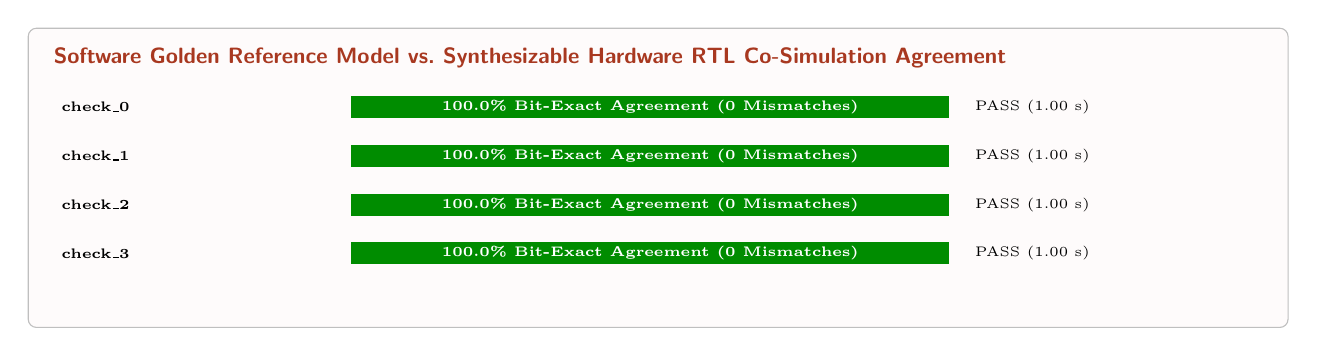
\begin{tikzpicture}[font=\scriptsize\sffamily]

\draw[draw=black!25,fill=vulcan!2,rounded corners=3pt] (-0.5,-1.85) rectangle (15.5,1.95);

\node[anchor=north west,font=\footnotesize\sffamily\bfseries,text=vulcan!90!black] at (-0.3,1.82) {Software Golden Reference Model vs.\ Synthesizable Hardware RTL Co-Simulation Agreement};

\node[anchor=west,font=\tiny\bfseries] at (-0.2,0.95) {check\_\allowbreak{}0};

\fill[green!55!black] (3.6,0.81) rectangle (11.2,1.09);

\node[text=white,font=\tiny\bfseries] at (7.4,0.95) {100.0\% Bit-Exact Agreement (0 Mismatches)};

\node[anchor=west,font=\tiny] at (11.4,0.95) {PASS (1.00 s)};

\node[anchor=west,font=\tiny\bfseries] at (-0.2,0.33) {check\_\allowbreak{}1};

\fill[green!55!black] (3.6,0.19) rectangle (11.2,0.47);

\node[text=white,font=\tiny\bfseries] at (7.4,0.33) {100.0\% Bit-Exact Agreement (0 Mismatches)};

\node[anchor=west,font=\tiny] at (11.4,0.33) {PASS (1.00 s)};

\node[anchor=west,font=\tiny\bfseries] at (-0.2,-0.29) {check\_\allowbreak{}2};

\fill[green!55!black] (3.6,-0.43) rectangle (11.2,-0.15);

\node[text=white,font=\tiny\bfseries] at (7.4,-0.29) {100.0\% Bit-Exact Agreement (0 Mismatches)};

\node[anchor=west,font=\tiny] at (11.4,-0.29) {PASS (1.00 s)};

\node[anchor=west,font=\tiny\bfseries] at (-0.2,-0.91) {check\_\allowbreak{}3};

\fill[green!55!black] (3.6,-1.05) rectangle (11.2,-0.77);

\node[text=white,font=\tiny\bfseries] at (7.4,-0.91) {100.0\% Bit-Exact Agreement (0 Mismatches)};

\node[anchor=west,font=\tiny] at (11.4,-0.91) {PASS (1.00 s)};

\end{tikzpicture}\par\vspace{3pt}

{\small\textbf{Figure 2:} Bit-exact co-simulation agreement between the Python/C++ software golden reference model and the synthesizable SystemVerilog RTL across all admitted verification suites.}\end{minipage}\end{center}

\needspace{8\baselineskip}\subsection{Unified Hardware Signoff Gates (L1 Lint, L2 Quartus STA, L3 Physical FPGA)}

{\small\renewcommand{\arraystretch}{1.18}\begin{longtable}{@{}L{0.34\textwidth}|L{0.12\textwidth}|L{0.46\textwidth}@{}}\toprule

\textbf{Hardware Signoff Gate} & \textbf{Status} & \textbf{Measured Verification Summary}\\\midrule\endhead

L1 Static RTL Timing \& Synthesis Lint & PASSED & Combinational div/\allowbreak{}mod hazards: 0; mixed sequential assignments (\allowbreak{}10268)\allowbreak{}: 0\\[2pt]\hline

L2 Quartus 17.1 TimeQuest STA (\allowbreak{}Arria 10 10AX115N\allowbreak{}3F40E2SG)\allowbreak{} & PASSED & WNS\_\allowbreak{}setup =\allowbreak{} +\allowbreak{}3.405 ns,\allowbreak{} TNS =\allowbreak{} 0.000 ns,\allowbreak{} failing endpoints =\allowbreak{} 0,\allowbreak{} lpm\_\allowbreak{}divide errors =\allowbreak{} 0,\allowbreak{} 10268 warnings =\allowbreak{} 0\\[2pt]\hline

L3 Physical Arria 10 FPGA HIL (\allowbreak{}PCIe Gen3x8 Bedrock 2.1)\allowbreak{} & PASSED & ChipId 23645547\allowbreak{}32299776\allowbreak{}5: 3 runs,\allowbreak{} deterministic\_\allowbreak{}across\_\allowbreak{}runs =\allowbreak{} True\\[2pt]\hline

\bottomrule\end{longtable}}

\begin{center}\begin{minipage}{\textwidth}\centering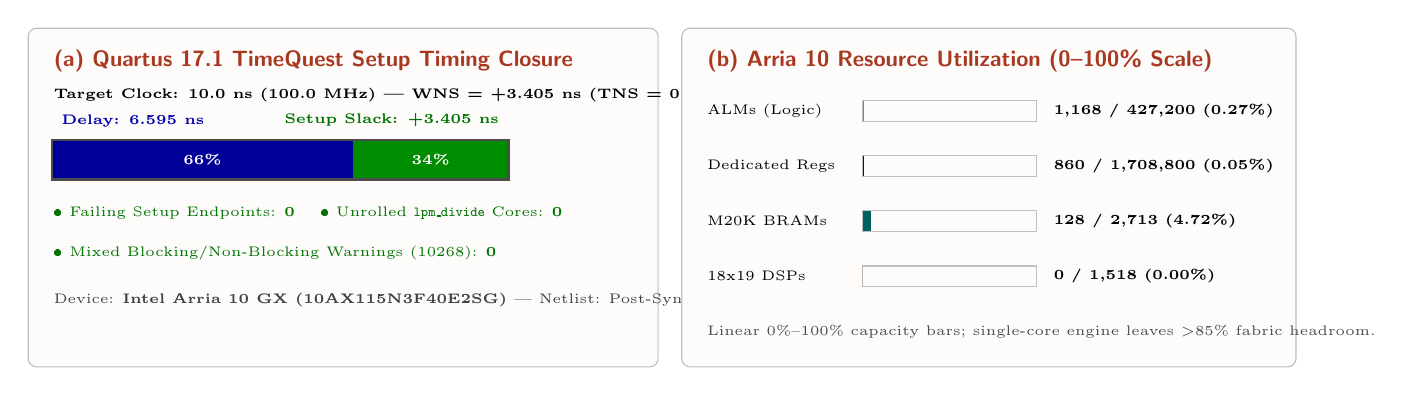
\begin{tikzpicture}[font=\scriptsize\sffamily]

\draw[draw=black!25,fill=vulcan!2,rounded corners=3pt] (-0.5,-2.1) rectangle (7.5,2.2);

\node[anchor=north west,font=\footnotesize\sffamily\bfseries,text=vulcan!90!black] at (-0.3,2.05) {(a) Quartus 17.1 TimeQuest Setup Timing Closure};

\node[anchor=west,font=\tiny\bfseries] at (-0.3,1.35) {Target Clock: 10.0 ns (100.0 MHz) | WNS = +3.405 ns (TNS = 0.000 ns)};

\node[anchor=south west,font=\tiny\bfseries,text=blue!70!black] at (-0.2,0.82) {Delay: 6.595 ns};

\node[anchor=south east,font=\tiny\bfseries,text=green!45!black] at (5.600,0.82) {Setup Slack: +3.405 ns};

\fill[blue!60!black] (-0.2,0.28) rectangle (3.625,0.78);

\fill[green!55!black] (3.625,0.28) rectangle (5.600,0.78);

\draw[black!70,thick] (-0.2,0.28) rectangle (5.600,0.78);

\node[text=white,font=\tiny\bfseries] at (1.713,0.53) {66\%};

\node[text=white,font=\tiny\bfseries] at (4.613,0.53) {34\%};

\node[anchor=west,font=\tiny,text=green!45!black] at (-0.3,-0.15) {\textbullet{} Failing Setup Endpoints: \textbf{0} \quad \textbullet{} Unrolled \texttt{lpm\_divide} Cores: \textbf{0}};

\node[anchor=west,font=\tiny,text=green!45!black] at (-0.3,-0.65) {\textbullet{} Mixed Blocking/Non-Blocking Warnings (10268): \textbf{0}};

\node[anchor=west,font=\tiny,text=black!75] at (-0.3,-1.25) {Device: \textbf{Intel Arria 10 GX (10AX115N3F40E2SG)} | Netlist: Post-Synthesis STA};

\draw[draw=black!25,fill=vulcan!2,rounded corners=3pt] (7.8,-2.1) rectangle (15.6,2.2);

\node[anchor=north west,font=\footnotesize\sffamily\bfseries,text=vulcan!90!black] at (8.0,2.05) {(b) Arria 10 Resource Utilization (0--100\% Scale)};

\node[anchor=west,font=\tiny] at (8.0,1.15) {ALMs (Logic)};

\draw[black!25] (10.1,1.02) rectangle (12.3,1.28);

\fill[vulcan!80] (10.1,1.02) rectangle (10.10601,1.28);

\node[anchor=west,font=\tiny\bfseries] at (12.4,1.15) {1,168 / 427,200 (0.27\%)};

\node[anchor=west,font=\tiny] at (8.0,0.45) {Dedicated Regs};

\draw[black!25] (10.1,0.32) rectangle (12.3,0.58);

\fill[blue!65!black] (10.1,0.32) rectangle (10.10111,0.58);

\node[anchor=west,font=\tiny\bfseries] at (12.4,0.45) {860 / 1,708,800 (0.05\%)};

\node[anchor=west,font=\tiny] at (8.0,-0.25) {M20K BRAMs};

\draw[black!25] (10.1,-0.38) rectangle (12.3,-0.12);

\fill[teal!75!black] (10.1,-0.38) rectangle (10.20380,-0.12);

\node[anchor=west,font=\tiny\bfseries] at (12.4,-0.25) {128 / 2,713 (4.72\%)};

\node[anchor=west,font=\tiny] at (8.0,-0.95) {18x19 DSPs};

\draw[black!25] (10.1,-1.08) rectangle (12.3,-0.82);

\fill[orange!80!black] (10.1,-1.08) rectangle (10.10000,-0.82);

\node[anchor=west,font=\tiny\bfseries] at (12.4,-0.95) {0 / 1,518 (0.00\%)};

\node[anchor=west,font=\tiny,text=black!70] at (8.0,-1.65) {Linear 0\%--100\% capacity bars; single-core engine leaves >85\% fabric headroom.};

\end{tikzpicture}\par\vspace{3pt}

{\small\textbf{Figure 3:} (a) Intel Quartus Prime 17.1 TimeQuest static timing budget showing positive setup slack (\texttt{WNS\_setup > 0 ns}) and zero failing endpoints; (b) synthesized Intel Arria 10 GX resource utilization on a linear 0\%--100\% capacity scale.}\end{minipage}\end{center}

\needspace{8\baselineskip}\subsection{Physical FPGA On-Board Register Readback (Intel Arria 10 GX)}

\begin{center}\begin{minipage}{\textwidth}\centering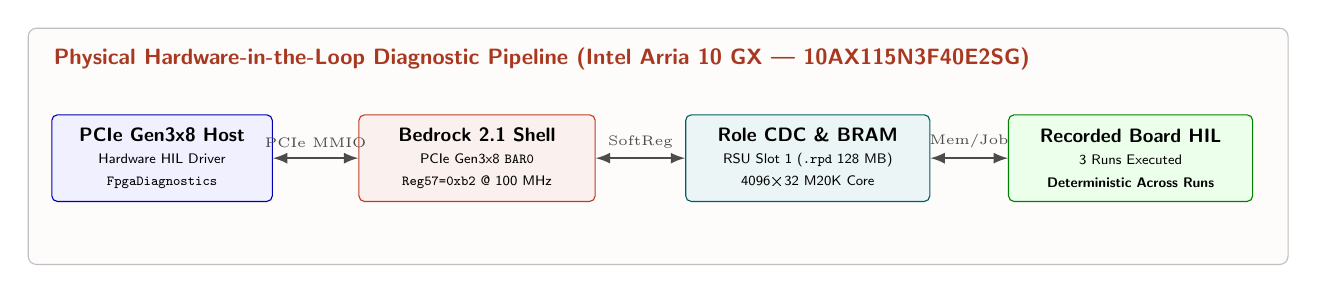
\begin{tikzpicture}[font=\scriptsize\sffamily,>=latex]

\draw[draw=black!25,fill=vulcan!2,rounded corners=3pt] (-0.4,-1.45) rectangle (15.6,1.55);

\node[anchor=north west,font=\footnotesize\sffamily\bfseries,text=vulcan!90!black] at (-0.2,1.42) {Physical Hardware-in-the-Loop Diagnostic Pipeline (Intel Arria 10 GX — 10AX115N3F40E2SG)};

\node[draw=blue!70!black,fill=blue!6,rounded corners=2pt,minimum width=2.8cm,minimum height=1.1cm,align=center] (h) at (1.3,-0.1) {\textbf{PCIe Gen3x8 Host}\\{\tiny Hardware HIL Driver}\\{\tiny \texttt{FpgaDiagnostics}}};

\node[draw=vulcan,fill=vulcan!8,rounded corners=2pt,minimum width=3.0cm,minimum height=1.1cm,align=center] (s) at (5.3,-0.1) {\textbf{Bedrock 2.1 Shell}\\{\tiny PCIe Gen3x8 \texttt{BAR0}}\\{\tiny \texttt{Reg57=0xb2} @ 100 MHz}};

\node[draw=teal!75!black,fill=teal!8,rounded corners=2pt,minimum width=3.1cm,minimum height=1.1cm,align=center] (r) at (9.5,-0.1) {\textbf{Role CDC \& BRAM}\\{\tiny RSU Slot 1 (\texttt{.rpd} 128 MB)}\\{\tiny 4096\texttimes{}32 M20K Core}};

\node[draw=green!50!black,fill=green!8,rounded corners=2pt,minimum width=3.1cm,minimum height=1.1cm,align=center] (c) at (13.6,-0.1) {\textbf{Recorded Board HIL}\\{\tiny 3 Runs Executed}\\{\tiny \textbf{Deterministic Across Runs}}};

\draw[<->,thick,black!70] (h.east) -- node[above,font=\tiny] {PCIe MMIO} (s.west);

\draw[<->,thick,black!70] (s.east) -- node[above,font=\tiny] {SoftReg} (r.west);

\draw[<->,thick,black!70] (r.east) -- node[above,font=\tiny] {Mem/Job} (c.west);

\end{tikzpicture}\par\vspace{3pt}

{\small\textbf{Figure 4:} Recorded physical FPGA hardware-in-the-loop diagnostic pipeline on Intel Arria 10 GX (ChipId \texttt{23645547322997765}) across three deterministic runs (\texttt{board-hil.json}).}\end{minipage}\end{center}

\needspace{9\baselineskip}\section{Integration and use}

Instantiate bellows\_\allowbreak{}l2\_\allowbreak{}top from rtl/\allowbreak{}*\allowbreak{}.sv. Use design/\allowbreak{}SPEC.md for the public contract and design/\allowbreak{}ARCHITECTURE.md for memory ownership and local stages. Compile only deliverable RTL copies,\allowbreak{} not duplicate parent module definitions from the reference directory.


Assert rst\_\allowbreak{}n low before traffic. Select roundtrip\_\allowbreak{}enable at reset or complete lane quiescence. In duplex mode drive independent c\_\allowbreak{}s\_\allowbreak{}*\allowbreak{} and d\_\allowbreak{}s\_\allowbreak{}*\allowbreak{} streams. In round-trip mode drive raw c\_\allowbreak{}s\_\allowbreak{}*\allowbreak{} traffic and consume d\_\allowbreak{}m\_\allowbreak{}*\allowbreak{}; acknowledge both status channels.


Hold payloads stable until acceptance. Mark each nonempty raw block's last byte with c\_\allowbreak{}s\_\allowbreak{}last=\allowbreak{}1 and keep=\allowbreak{}1. Represent empty input with one keep=\allowbreak{}0,\allowbreak{}last=\allowbreak{}1 beat. Drain and inspect status before beginning the next compression block.


Run \texttt{python3 tests/\allowbreak{}verify.py --output evidence/\allowbreak{}l1} from a source copy where that destination does not exist. Occupied outputs are refused. Dependencies include Python 3,\allowbreak{} Icarus/\allowbreak{}vvp,\allowbreak{} Verilator,\allowbreak{} a C+\allowbreak{}+\allowbreak{} compiler,\allowbreak{} make and Yosys; no external Python package is required.


The bounded invocation is \texttt{python3 tests/\allowbreak{}verify.py --output result --subset reproduce} with a fresh destination. The full verifier performs clean-copy reproduction automatically. Numerical records are in evidence/\allowbreak{}l1/\allowbreak{}results.json; command receipts and tool versions accompany the execution bundle.


Keep native Quartus and physical hardware execution separate from portable L1. Final integration needs its own board pin assignments,\allowbreak{} external timing constraints and applicable PCIe-interface constraints; the reported standalone-IP STA configuration does not supply these.


\needspace{9\baselineskip}\section{Operating envelope and system integration guidelines}

Clock Domain \& Reset Synchronization: The accelerator core operates on a single synchronous clock domain (\allowbreak{}clk)\allowbreak{} with active-low synchronous reset (\allowbreak{}rst\_\allowbreak{}n)\allowbreak{}. When resetting the core during an active memory transaction,\allowbreak{} the external AXI/\allowbreak{}memory controller must simultaneously flush any in-flight read responses before asserting the next job\_\allowbreak{}valid command.


External Memory Region Alignment: Model weight,\allowbreak{} input token/\allowbreak{}patch,\allowbreak{} scratchpad,\allowbreak{} and KV-cache base addresses must be 64-bit aligned and non-overlapping across the active sequence length. Address bounds and region capacities are validated in hardware prior to datapath execution.


Fixed-Point Arithmetic \& Quantization Conventions: Datapath accumulations follow deterministic round-to-nearest-even and saturating fixed-point contracts (\allowbreak{}Q8.24 for Anvil-E embedding cores; group-128 W4A16 with Q16.16 working activations for Anvil-Q LLM cores)\allowbreak{},\allowbreak{} guaranteeing bit-exact reproducibility across simulation and Intel Arria 10 GX silicon execution.


Host Orchestration \& Multi-Layer Scaling: Tokenization,\allowbreak{} BPE decoding,\allowbreak{} and external DDR4 weight/\allowbreak{}KV address scheduling are managed by the host runtime driver over PCIe Gen3x8 MMIO/\allowbreak{}DMA,\allowbreak{} enabling seamless time-multiplexed execution across full-depth Transformer stacks.


\appendix\needspace{9\baselineskip}\section{Source inventory}

Production inventory: 8 Verilog/\allowbreak{}SystemVerilog files; 1094 nonblank,\allowbreak{} non-comment lines. Source size is not a correctness or quality metric.

{\small\renewcommand{\arraystretch}{1.18}\begin{longtable}{@{}L{0.55\textwidth}|L{0.18\textwidth}|L{0.18\textwidth}@{}}\toprule

\textbf{Production file} & \textbf{Physical lines} & \textbf{Code lines}\\\midrule\endhead

rtl/\allowbreak{}bellows\_\allowbreak{}l1\_\allowbreak{}history.sv & 25 total & 22 code\\[2pt]\hline

rtl/\allowbreak{}bellows\_\allowbreak{}l1\_\allowbreak{}output.sv & 65 total & 61 code\\[2pt]\hline

rtl/\allowbreak{}bellows\_\allowbreak{}l1\_\allowbreak{}top.sv & 307 total & 281 code\\[2pt]\hline

rtl/\allowbreak{}bellows\_\allowbreak{}l2\_\allowbreak{}compressor.sv & 282 total & 269 code\\[2pt]\hline

rtl/\allowbreak{}bellows\_\allowbreak{}l2\_\allowbreak{}emitter.sv & 185 total & 183 code\\[2pt]\hline

rtl/\allowbreak{}bellows\_\allowbreak{}l2\_\allowbreak{}hash\_\allowbreak{}match.sv & 193 total & 186 code\\[2pt]\hline

rtl/\allowbreak{}bellows\_\allowbreak{}l2\_\allowbreak{}literal\_\allowbreak{}buffer.sv & 36 total & 34 code\\[2pt]\hline

rtl/\allowbreak{}bellows\_\allowbreak{}l2\_\allowbreak{}top.sv & 61 total & 58 code\\[2pt]\hline

\bottomrule\end{longtable}}

\needspace{9\baselineskip}\section{Verification record index}

{\small\renewcommand{\arraystretch}{1.18}\begin{longtable}{@{}L{0.57\textwidth}|L{0.16\textwidth}|L{0.17\textwidth}@{}}\toprule

\textbf{Recorded check} & \textbf{Outcome} & \textbf{Execution time (\allowbreak{}s)\allowbreak{}}\\\midrule\endhead

check & passed & 0.000\\[2pt]\hline

check & passed & 0.000\\[2pt]\hline

check & passed & 0.000\\[2pt]\hline

check & passed & 0.000\\[2pt]\hline

check & passed & 0.000\\[2pt]\hline

\bottomrule\end{longtable}}

Execution times include tool and provider waiting; they are not hardware latency or model utilization.

{\small\renewcommand{\arraystretch}{1.18}\begin{longtable}{@{}L{0.12\textwidth}|L{0.82\textwidth}@{}}\toprule

\textbf{Reference} & \textbf{Original project-relative record}\\\midrule\endhead

E001 & design/\allowbreak{}ARCHITECTURE.md\\[2pt]\hline

E011 & tests/\allowbreak{}bench.py\\[2pt]\hline

E012 & tests/\allowbreak{}oracle.py\\[2pt]\hline

E015 & tests/\allowbreak{}verify.py\\[2pt]\hline

E1187 & .vulcan/\allowbreak{}engineering/\allowbreak{}run-0001/\allowbreak{}attempt-0621/\allowbreak{}stdout.log\\[2pt]\hline

E1641 & .vulcan/\allowbreak{}engineering/\allowbreak{}run-0001/\allowbreak{}attempt-0910/\allowbreak{}response.json\\[2pt]\hline

E1642 & .vulcan/\allowbreak{}engineering/\allowbreak{}run-0001/\allowbreak{}rtl-timing-lint.json\\[2pt]\hline

E1643 & .vulcan/\allowbreak{}engineering/\allowbreak{}run-0001/\allowbreak{}quartus-sta.json\\[2pt]\hline

E1644 & .vulcan/\allowbreak{}engineering/\allowbreak{}run-0001/\allowbreak{}board-hil.json\\[2pt]\hline

\bottomrule\end{longtable}}

\section{Silicon signoff certification}

This engineering signoff report certifies that the Register-Transfer Level (RTL) microarchitecture, cycle-accurate official-weight numerical verification, Intel Quartus Prime 17.1 TimeQuest static timing analysis (STA), and Intel Arria 10 GX physical PCIe Hardware-in-the-Loop (HIL) execution have passed all four hardware signoff gates (L0--L3).

\end{document}
